%**********************************************************************
% Base layout + including standard packages
%**********************************************************************
\documentclass[a4paper,12pt]{report}


%**********************************************************************
% TODO for EVERYONE:
% READ "Instructions for composing degree papers" (E, short version)
% READ "Richtlinien Pruefungs- u. Abschlussarbeiten" (D, long version)
%**********************************************************************


%**********************************************************************
% YOUR SETTINGS - START
%**********************************************************************

% About your study degree programme
\def \study{SWD} % possible options: ITM, SWD, IRM, IMS

% More about you and your thesis:
\def \title{Code Quality und Einsatz der Statischen Code Analyse für weitere Auswertungen und Präsentationen der Daten}
\def \subtitle{}
\def \yourName{Lukas Wechtitsch}
\def \yourIdentifier{1710418051}
\def \yourPlace{Kapfenberg}
\def \submissionDate{Februar 2020}  % month year. e.g. June 2017
\def \yourAdvisor{Johannes Feiner}  

% ITM/SWD/IRM: you could possibly write in German.
\def \yourLanguage{german} % po ssible options: german, english  

%**********************************************************************
% YOUR SETTINGS - END
%**********************************************************************



% LaTeX preamble = include a lot of packages, configure latex settings
%**********************************************************************
% Various LaTeX packages
%**********************************************************************


% 
\usepackage{ifthen}

% you might need some mathematical expressions:
\usepackage{amsmath}

% with package babel we allow to use language english and german
\usepackage[english, german]{babel}

% allows direct input of special chars
\usepackage[utf8]{inputenc}  

% permits to set space between lines
\usepackage{setspace}  	

% ensure proper appearance of all fonts in pdf:
\usepackage[T1]{fontenc}

% lmodern after T1 fontenc (_may_ be required)
% lmodern = Latin Modern fonts
%\usepackage{lmodern}  	

%\usepackage{times} -- obsolete; use:
% Times as default text font, maths support
\usepackage{mathptmx}  	
% provides bold font (required for syntax highlighting in listings)
\usepackage{courier}  	

% enables table cells to span multiple rows
\usepackage{multirow}  
% paragraphs: no indentation at beginning, but spacing between  
\usepackage{parskip}  	

% for figures
\usepackage[pdftex]{graphicx}
% implicit file name extensions for embedded figures 
% so we do not need to specify the extension on inclusion
\DeclareGraphicsExtensions{.pdf,.jpg,.png}

% for flexible tables (e.g. auto resizing to page width) 
\usepackage{tabularx}

%**********************************************************************
% Including non-standard packages
%**********************************************************************

\usepackage{acronym}

% http://en.wikibooks.org/wiki/LaTeX/Colors
\usepackage[usenames,dvipsnames,table]{xcolor}
% we define a few custom colors  
\definecolor{gray20}{gray}{0.8}
\definecolor{gray5}{gray}{0.95}
\definecolor{olivegreen30}{RGB}{155,187,89}  

\usepackage{alltt}

% for code snippets, embedded as "listings"
\usepackage{listings}
% we set a few defaults:
\lstset{numbers=left, 
        basicstyle=\footnotesize\ttfamily,  
        showstringspaces=false,
        % numbers=none           % line numbering
        captionpos=b,            % caption at bottom
        breaklines=false, 
        numbersep=5pt
}
  
% the page layout (geometry), as defined by FH guidelines:
\usepackage[top=3cm, 
            bottom=3cm, 
            left=3.5cm, 
            right=3cm]
           {geometry}

\usepackage[super]{nth}     % 1st, 2nd, 3rd,...

%\usepackage{paralist}   	% inline lists
%\usepackage{mdwlist}
\usepackage{enumitem}

% e.g. for "floating" listings (no fixed anchor in text)
\usepackage{float}     
\floatstyle{plain}
\restylefloat{figure}
% e.g. to show two (floating) images side-by-side
\usepackage{subfig}

% add copyright information to figures
\usepackage{copyrightbox} 



% symbols such as \texttimes and \texteuro
\usepackage{textcomp}  
% math. symbols from the American Mathematical Society  
%\usepackage{amssymb}  	


% chapter heading styles
\usepackage[Lenny]{fncychap}  

% for \enquote, \textquote, \blockquote...
\usepackage{csquotes}       
\graphicspath{ {images/} }
% how to create simple helper commands (LaTeX "macros"):
% e.g. in text you will write ... \TODO{add reference} ...
\newcommand{\TODO}[1]
{
{\textcolor{red}{[TODO: #1]}}
}


% how to create/style more complex new commands:
% e.g. \chapquote{Phone home!}{by E.T.}
% BEGIN: chapquote
\newcommand{\chapquote}[2]  
{%
\begin{quote}
\emph{%
``#1''%
}%
\begin{flushright}
{\scriptsize \sffamily [#2]}%
\end{flushright}
\end{quote}
}
% END: chapquote

% Biblatex = bibliography for LaTeX
% ---------------------------------------------------------------------
% context sensitive quotation; recommended for usage with Biblatex
\usepackage{csquotes}  	
% Note: \date, \origdate, \eventdate, and \urldate 
%       require "yyyy-mm-dd" format,
%       so "dd" or "mm-dd" may be omitted
\usepackage[backend=biber,
            urldate=long,  	        % default: short, e.g. 08/15/2010
            style=authoryear-icomp, % Harvard citation style
            backref,                % if you like (cit. on p. 2)
            % sorting=nty  	        % this is default: sort by name, title, year
            % sortlocale=de_DE      % set according to your needs
            natbib=true,  	        % use natbib compatible citation commands
                                    % do _not_ use package natbib!
            maxbibnames=1000,  	    % show all authors in the bibliography
]{biblatex}
% Note the default option: ibidpage=true for ibid / ebd ("ebenda")

% We enforce strict Harvard style: 
% The URL date default is "(Visited on ...);" => so:
%     BibTeX entries such as:
%      url = {http://...},
%      urldate = {2015-03},
%       urldate = {2015},
%       urldate = {2015-03-31},
%     shall be printed as
%      Available from: <http://...> [March 2015]
\DeclareFieldFormat{urldate}{\mkbibbrackets{#1}}
\DeclareFieldFormat{url}{Available\space from\addcolon\space \url{#1}}

% Add one (or multiple) file(s) with bibliography entries:
\addbibresource{references.bib}


% ---------------------------------------------------------------------

\usepackage[  	      % hyperref should be last package loaded
    pdftex,  	      % driver
    pdftitle={bac1_wechtitsch},
    pdfsubject={Master's Thesis},
    pdfauthor={<your name>},
    breaklinks,  	  % permits line breaks for long links
    bookmarks,  	      % create Adobe bookmarks
    bookmarksnumbered,% ... and include section numbers
    linktocpage,  	  % the page number (not the text) is link on TOC
    colorlinks,  	  % 
    linkcolor=black,  % normal internal links;
    anchorcolor=black,% don't make scientific papers too colourful
    citecolor=black,
    urlcolor=blue,  	  % quite common
    pdfstartview={Fit},  % "Fit" fits the page to the window
    pdfpagemode=UseOutlines,  % open bookmarks in Acrobat
    plainpages=false, % avoids duplicate page number problem
    pdfpagelabels,
  ]{hyperref}

%**********************************************************************
% Layout adjustments
%**********************************************************************

% page layout (header/footer and page numbers)
%\pagestyle{empty}
\pagestyle{headings}
%\pagestyle{fancy}

% settings for structure and numbering 
%  we allow three levels within text:  1.2.1 
\setcounter{secnumdepth}{3}
%  but we show two levels in TOC: 1.2
\setcounter{tocdepth}{1}

% footnotes: no indent, hanging
\usepackage[hang,flushmargin]{footmisc}

%**********************************************************************
% LaTeX macros and commands
%**********************************************************************

% new command to start a chapter (no page number)
\newcommand{\chapterstart}{\thispagestyle{empty}}

% command "\chapterend" to close a chapter 
% (flush, i.e. print remaining figures and tables)
\newcommand{\chapterend}
           {\newpage{
              \pagestyle{empty}
               \cleardoublepage
             }
           }

% You might define support for further programming languages
% when using listings
\usepackage{color}
\definecolor{lightgray}{rgb}{.9,.9,.9}
\definecolor{darkgray}{rgb}{.4,.4,.4}
\definecolor{purple}{rgb}{0.65, 0.12, 0.82}
\lstdefinelanguage{JavaScript}{
  keywords={break, case, catch, continue, debugger, default, delete, do, else, false, finally, for, function, if, in, instanceof, new, null, return, switch, this, throw, true, try, typeof, var, void, while, with},
  morecomment=[l]{//},
  morecomment=[s]{/*}{*/},
  morestring=[b]',
  morestring=[b]",
  ndkeywords={class, export, boolean, throw, implements, import, this},
  keywordstyle=\color{blue}\bfseries,
  ndkeywordstyle=\color{darkgray}\bfseries,
  identifierstyle=\color{black},
  commentstyle=\color{purple}\ttfamily,
  stringstyle=\color{red}\ttfamily,
  sensitive=true
}


% new environment for smaller paragraphs
% e.g. \begin{spar}A paragraph with some indentation.\end{spar}
\newenvironment{spar}
{\begingroup \leftskip 0.7cm \rightskip\leftskip}
{\par \endgroup}
% ^^^ must be set here (or use empty line)

%**********************************************************************
% Special hyphenation rules
%**********************************************************************

\hyphenation{JOANNEUM}  	% extend to your needs


%**********************************************************************
% Different settings for ITM / SWD / IRM / IMS
%**********************************************************************


% ITM = Internettechnik
% ------------------------
\ifthenelse{\equal{\study}{ITM}}{
  \def \theStudyProgramme {Internettechnik}
  \def \isBachelorThesis {}
}
%\fi

% SWD = Software Design
% ------------------------
\ifthenelse{\equal{\study}{SWD}}{
  \def \theStudyProgramme {Software Design}
  \def \isBachelorThesis {}
}

% IRM = IT-Recht & Management
% -------------------------------
\ifthenelse{\equal{\study}{IRM}}{
  \def \theStudyProgramme {IT-Recht \& Management}
  \def \isMasterThesis {}
}

% IMS = IT & Mobile Security
% ------------------------------
\ifthenelse{\equal{\study}{IMS}}{
  \def \theStudyProgramme {IT \& Mobile Security}
  \def \isMasterThesis {}
}


 


%**********************************************************************
% Structure of thesis: inclusion of chapters
%**********************************************************************
\ifthenelse{\equal{\yourLanguage}{german}}{

  \begin{document}\selectlanguage{german}

}{ % else: default language = english

  \begin{document}\selectlanguage{english}
}

%**********************************************************************
% right side, if two-sided
\chapterend

\begin{titlepage}

\begin{center}
% scale image according to the actual logo you use
% official JPG ist way too large, so [height=2.5cm] is required
% official EPS, converted to PDF:
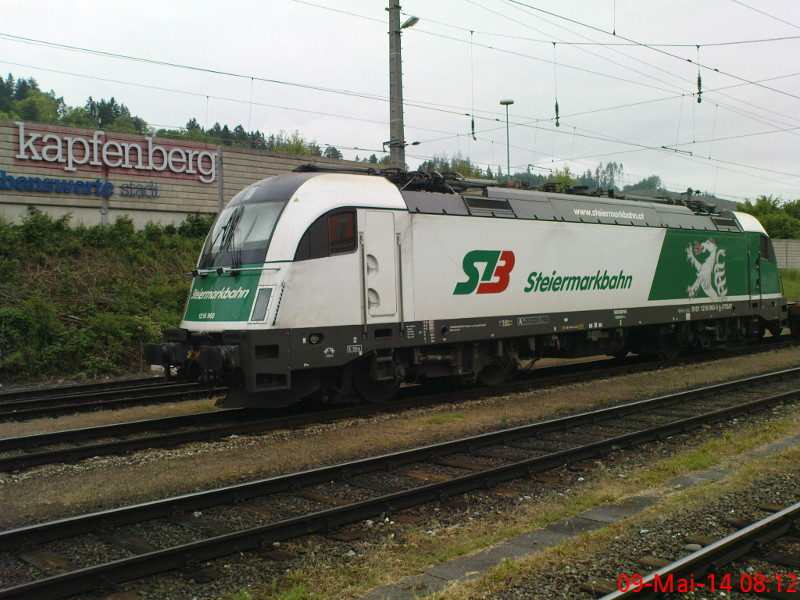
\includegraphics[height=1cm]{images/engine.jpg}
\hfill

% the actual title
\mbox{}\vfill

  \large

  {\huge\bf \title \par}
  \subtitle
  \vspace{2.0cm}
  
\ifdefined\isMasterThesis % MA

  \ifthenelse{\equal{\yourLanguage}{german}}{ % German Version 

   {\bf Masterarbeit}\\
    zur Erlangung des akademischen Grades\\
   
    \ifthenelse{\equal{\study}{IRM}}{ % IRM Master of Arts
  
      {\bf Master of Arts in Business (MA)}\\
      eingereicht am\\
      Fachhochschul-Studiengang {\bf \theStudyProgramme \\}
  
    }{  % else: IMS = Master of Science
      
      {\bf Master of Science in Engineering (MSc)}\\
      eingereicht am\\
      Fachhochschul-Studiengang {\bf \theStudyProgramme \\}
      
   }

  }{ % English Version 

    {\bf Master Thesis}\\
    submitted in conformity with the requirements for the degree of\\
   
    \ifthenelse{\equal{\study}{IRM}}{ % IRM Master of Arts
  
      {\bf Master of Arts in Business (MA)}\\
      Master's degree programme {\bf \theStudyProgramme \\}
  
    }{  % else: IMS = Master of Science
      
      {\bf Master of Science in Engineering (MSc)}\\
      Master's degree programme {\bf \theStudyProgramme \\}
      
   }

  } 
\else % BA
  
  \ifthenelse{\equal{\yourLanguage}{german}}{ % German Version 
  
  {\bf Bachelorarbeit}\\
  zur Erlangung des akademischen Grades\\
  {\bf Bachelor of Science in Engineering (BSc)}\\
  
  eingereicht am\\
  Fachhochschul-Studiengang {\bf \theStudyProgramme \\}

  }{ % English Version 
  
  {\bf Bachelor Thesis}\\
  submitted in conformity with the requirements for the degree of\\
  {\bf Bachelor of Science in Engineering (BSc)}\\
  Bachelor's degree programme {\bf \theStudyProgramme \\}

  }

\fi
  
  \vspace{0.5cm}

 FH JOANNEUM  (University of Applied Sciences), Kapfenberg

  \vspace{1.5cm}

  \mbox{}

  \ifthenelse{\equal{\yourLanguage}{german}}{ % German Version

  {\bf Betreuer/in: \yourAdvisor\\
   % Zweit-/Firmenbetreuer/in: <Vorname Zuname; Firmenname>

  eingereicht von: \yourName\\
  Personenkennzahl: \yourIdentifier}
  
  
  }{ % English Version 

  {\bf supervisor: \yourAdvisor\\ 
  % second supervisor: <firstname lastname; company>

  submitted by: \yourName\\
  personal identifier: \yourIdentifier}
  
  }

  \vspace{1.5cm}

   \submissionDate
  
  \vspace{1.5cm}


\end{center}

\vfill\mbox{}


\end{titlepage}



%**********************************************************************

%**********************************************************************

% right side
\chapterend

\begin{titlepage}

%-t-\parindent0pt
%-t-\parskip1.5ex plus.5ex minus.5ex

\begin{center}\large\bf

\ifthenelse{\equal{\yourLanguage}{german}}{
%**********************************************************************
% Verpflichtend zu unterzeichnende Ehrenwörtlichen Erklärung:
%**********************************************************************
Ehrenwörtliche Erklärung
\end{center}

Ich erkläre ehrenwörtlich, dass ich die vorliegende
\ifdefined\isMasterThesis
Masterarbeit
\else
Bachelorarbeit
\fi
selbstständig angefertigt und die mit ihr verbundenen Tätigkeiten selbst erbracht habe. Ich erkläre weiters, dass ich keine anderen als die angegebenen Hilfsmittel benutzt habe. Alle aus gedruckten, ungedruckten oder dem Internet im Wortlaut oder im wesentlichen Inhalt übernommenen Formulierungen und Konzepte sind gemäß den Regeln für gutes wissenschaftliches Arbeiten zitiert und durch Fußnoten bzw. durch andere genaue Quellenangaben gekennzeichnet.

Die vorliegende Originalarbeit ist in dieser Form zur Erreichung eines akademischen Grades noch keiner anderen Hochschule vorgelegt worden. Diese Arbeit wurde in gedruckter und elektronischer Form abgegeben. Ich bestätige, dass der Inhalt der digitalen Version vollständig mit dem der gedruckten Version übereinstimmt.

Ich bin mir bewusst, dass eine falsche Erklärung rechtliche Folgen haben kann.


%**********************************************************************
% Verpflichtend zu unterzeichnende Ehrenwörtlichen Erklärung -- END
%**********************************************************************
 
}{ % else in English (default)

%**********************************************************************
% Obligatory signed declaration:
%**********************************************************************
Formal declaration
\end{center}

I hereby declare that the present 
\ifdefined\isMasterThesis 
master's thesis 
\else
bachelor's thesis
\fi
was composed by myself and that the work contained 
herein is my own. I also confirm that I have only used the specified 
resources. All formulations and concepts taken verbatim or in substance 
from printed or unprinted material or from the Internet have been 
cited according to the rules of good scientific practice and indicated
by footnotes or other exact references to the original source.

The present thesis has not been submitted to another university 
for the award of an academic degree in this form. This thesis 
has been submitted in printed and electronic form. I hereby 
confirm that the content of the digital version is the same 
as in the printed version.

I understand that the provision of incorrect information may 
have legal consequences.

%**********************************************************************
% Obligatory signed declaration -- END
%**********************************************************************

}% end of english version of formal declaration


\vspace{1,5cm}
\yourPlace, \submissionDate

\flushright
\vspace{15mm}
% Here your name serves as signature
\yourName


\end{titlepage}





%**********************************************************************

%**********************************************************************

%---------------------------------------------------
% NOTE:
% English version of the abstract is always required 
% (even for German BA/MAs)
%---------------------------------------------------

% right side/flush
\chapterend

\begin{titlepage}

\begin{otherlanguage}{english} 
\begin{abstract} % Abstract

Code quality is an important part in the process of software development. Static code analysis is a possibility to reach a good code quality. This is the analysis of code during the compile time. The result of this analysis is the finding of bugs, code smells, security issues and other problems. The tools, that perform the static code analysis, presents the results in various forms: In desktop or web applications or in development environments. There are some different problems in these presentations, so that the developers’ code is not permanently improved. These are problems like not saving the data permanently, therefore the data can not be analyzed further. Other problems are the missing of individuality or the imperfect presentation of data.

The question is, how the information of the static code analysis should be presented, and further analysis could help the developers permanently. A web application and a plugin should solve the problem. In the web application the data is presented in different forms. The Plugin will import the data from the developers’ project into a database. 

The evolution with test subjects and the comparison with other solutions show the potential of display the information in different ways, to improve the code of the developers. The presentations include forms like visualizations, presenting tables and other possibilities to improve the code quality. 


\end{abstract}
\end{otherlanguage}


\end{titlepage}


%---------------------------------------------------
% NOTE:
% German version of the abstract "Zusammenfassung"
% is ONLY required (for German BA/MAs)
%---------------------------------------------------

\ifthenelse{\equal{\yourLanguage}{german}}{
\begin{titlepage}
\begin{otherlanguage}{german}
\begin{abstract}  % Zusammenfassung

%Zusammenfassung. (Sollte das gesamte Werk enthalten, also das spannende Problem, den gewählten --neuartigen-- Lösungsansatz und natürlich vor allem die erreichten Resultate).

Ein wichtiger Punkt in der Softwareentwicklung ist die Code Qualität. Ein Mittel, um eine hohe Code Qualität zu erreichen, ist die Statische Code Analyse. Unter der Statischen Code Analyse versteht man die Analyse des Codes zur Übersetzungszeit. Diese Analyse wird durchgeführt um Fehler, Sicherheitslücken, Code Smells und andere Probleme im Code ausfindig zu machen. Die Tools, die die Statische Code Analyse durchführen, präsentieren die Ergebnisse in verschiedenen Formen: In einer Desktopapplikation, Webapplikation oder in der Entwicklungsumgebung. Hierbei gibt es verschiedene Probleme, sodass der Code der Entwicklerinnen und Entwickler nicht dauerhaft verbessert wird. Eines der Probleme ist die fehlende dauerhafte Speicherung der Fehler. So können auch keine weiteren Analysen durchgeführt werden. Weitere Probleme sind die fehlende Individualität oder die oft rudimentär und mangelnden Anzeigen der Informationen.

Dadurch stellt sich die Frage, wie mit den Daten der Statischen Code Analyse weiterreichende Analysen und dauerhafte Informationsübersichten erstellt werden können und welche Möglichkeiten es gibt, daraus einen langfristigen Vorteil für die Entwicklerin oder den Entwickler zu erreichen. 
Dazu werden eine Webapplikation und ein Plugin entwickelt. In der Webapplikation werden die Daten der Statischen Code Analyse in verschiedenen Formen aufbereitet. Das Plugin kann von den Entwicklerinnen und Entwicklern in das Projekt eingebunden werden, sodass die Daten der Codeanalyse in die Datenbank importiert werden können.

Die Evaluierung anhand Testpersonen und Vergleiche mit herkömmlichen Lösungen zeigen, dass die Ergebnisse der Code Analyse in verschiedenen Arten angezeigt und weiter verwendet werden um den Code der Entwicklerinnen und Entwickler nachhaltig zu verbessern. Die geschieht mittels Visualisierungen, Tabellen und weiteren Möglichkeit zur Verbesserung der Code Qualität.

\end{abstract}
\end{otherlanguage}
\end{titlepage}

}{ % English Version 
% already inserted above
}

%**********************************************************************

% %**********************************************************************

% Optional: add acknowledgement
\chapterend

\begin{titlepage}

\begin{center}\large\bf

\ifthenelse{\equal{\yourLanguage}{german}}{ % German Version
 Danksagung 
}{ % English Version
 Acknowledgement 
}
\end{center}
Thanks to \ldots

\end{titlepage}


%**********************************************************************
 % optional
\chapterend

\pagenumbering{roman}  	% roman page numbers for title pages





\tableofcontents            % TOC = Table-of-Contents
  
% OPTIONALLY, adding single entries to TOC: 

% Adding entry "List of Figures / Abbildungsverzeichnis" to TOC
\clearpage
\addcontentsline{toc}{chapter}{\listfigurename} 
\listoffigures

% Adding entry "List of Tables / Tabellenverzeichnis" to TOC
%\clearpage
%\addcontentsline{toc}{chapter}{\listtablename}
%\listoftables 

% Adding entry "List of Code Snippets" to TOC
\clearpage
\addcontentsline{toc}{chapter}{List of Code Snippets}
\lstlistoflistings

\chapterend





\pagenumbering{arabic}  % ... for ordinary chapters
\onehalfspacing

% Add chapters as required. For example 

\chapter{Einleitung}

\section{Problemstellung}
Code Quality ist ein oft unterschätzter Teil der Softwareentwicklung. Viele Bugs und Sicherheitslücken können durch eine gesteigerte Code Quality vermieden werden. Um die Code Quality in einem Software-Projekt zu verbessern, werden Hilfsmittel eingesetzt, wie Tools für die Statische Code Analyse. Statische Code Analysen überprüfen den Code während der Übersetzungszeit (Compiler Übersetzung) und zeigen auftretende Fehler und verschiedene Warnungen auf. Die daraus folgenden Informationen sind aber rudimentär, d.h. text-basiert und unübersichtlich. Ebenso wird eine Verbesserung des Codestils nur schwer erreicht, da die Informationen nicht dauerhaft verfügbar sind. Die Analysen gestalten sich daher nur als Momentaufnahme aus dem Code. 

\section{Zielsetzung und Forschungsfragen}

Dadurch stellt sich die Frage, wie mit den Daten der Statischen Code Analyse weiterreichende Analysen und dauerhafte Informationsübersichten erstellt werden können und welche Möglichkeiten es gibt, daraus einen langfristigen Vorteil für die Entwicklerin oder den Entwickler zu erreichen. Das Ziel ist es daher, verschiedene Analyse- und Aufbereitungsmöglichkeiten der Daten zu entwickeln, die der Benutzerin oder den Benutzer bei der Verbesserung in der Entwicklung unterstützen und dadurch die Code Qualität in Projekten langfristig erhöht wird.

\subsection{Methodik} 

Mithilfe einer Webapplikation werden Daten verschiedener Code-Analyse-Tools ausgewertet und präsentiert. Dazu werden in mehreren verschiedenen Projekten diese Tools eingesetzt werden. Die Analysen in der Webapplikation bauen auf diese Daten auf, die mithilfe eines Plugins und eines Datenbank-Imports gespeichert werden. Die Präsentation und Visualisierungen sollen unabhängig von den eingesetzten Tools sein.

Um die Effizienz, Anwendung und Mehrwertigkeit der Webapplikation und der Analysen festzustellen, werden Tests und Anwendungsfälle mit verschiedenen Entwicklerinnen und Entwicklern durchgeführt. Die durchführenden Benutzerinnen und Benutzer sollen hierbei einen unterschiedlichen Wissenstand im Bereich der Softwareentwicklung aufweisen, sodass die Ergebnisse nur auf der Webapplikation und nicht auf Wissen über bestimmte Tools und Fehler basieren. 


Beim Durchführen der Tests muss darauf geachtet werden, dass sich das Testsetup und die Testumgebung nicht unterscheidet. Die Ergebnisse der Tests werden protokolliert. Im Test können die Testpersonen mit der Applikation direkt und interaktiv arbeiten. Dies geschieht im Rahmen eines Interviews, wo die Anwenderinnen und Anwender Erfahrungen mit der Applikation, Kritikpunkte und Vorschläge einbringen können. Der Test beginnt mit einer zurückgesetzten Datenbank und einem leeren Frontend. Mittels einer Bildschirmübertragung, bei der die Testpersonen auch die Steuerung des Computers übernehmen können, wird der Test durchgeführt.
Der Test beinhaltet die Beantwortung von vorgefertigten Fragen, das Ausführen der Funktionen, das Suchen von angezeigten Fehlern sowie offenes Feedback.
Die Tests finden online statt haben einen Zeitrahmen von 30 bis 45 Minuten. 
\subsection{Kriterien} 
Testpersonen evaluieren die Arbeit anhand folgender Kriterien und Punkte:
\begin{itemize}
\item Einfachheit \\ Die Verwendung der Applikation soll unkompliziert und einfach geschehen. Dies beinhaltet den Einbau des Plugins, das Starten der Applikation und die Auswahl der richtigen Daten.
\item Übersicht \\ Im Frontend sollen alle wichtigen Informationen übersichtlich und gut lesbar aufbereitet werden können. Ebenso kann der Benutzer bestimmte Daten selektieren, um einen genaueren Überblick zu bekommen.
\item Unterstützungshilfe \\ Durch die Visualisierungen, Tabellen und andere Funktionalitäten soll der Benutzer eine Unterstützung bei der Entwicklung bekommen.
\item Individualität \\ Die Applikation soll für die Arbeit der Benutzer und deren eingesetzten Code Analyse Tools verfügbar und kompatibel sein. 
\item Performance \\ Die Benutzerin oder der Benutzer kann nach einsetzen der Applikation schnell seine Daten einsehen.
\item Verständlichkeit \\ Die Visualisierungen und Funktionalitäten sollen für die Benutzerinnen und Benutzer ohne Hilfestellungen verständlich sein und sollen daher ohne Probleme verwendet und angewandt werden können.
\end{itemize}

Ebenso werden anhand dieser Kriterien die Unterschiede zu herkömmlichen Lösungen erarbeitet. Die Arbeit ist erfolgreich, wenn diese Kriterien für die Testpersonen zutreffen. 

   % framing the problem 
                                     % research questions
                                     % hypothesis
                                     % method


\chapter{Stand der Technik}
\section{Andere Lösungen}
Das Ziel des praktischen Teils der Bachelorarbeit ist es, die Informationen der Statischen Code Analyse übersichtlicher, dauerhafter und benutzerfreundlicher zu präsentieren. Hierbei gibt es ähnliche bereits bestehende Lösungen, deren Probleme im Punkt 2.3.2 Probleme aufgezeigt werden: 

\subsection{Entwicklungsumgebungen}
Bestehende Entwicklungsumgebungen zeigen die Informationen und Warnung bezüglich Fehler und Regelverletzungen zur Übersetzungszeit auf. Dies geschieht in der Zeile bzw. bei der Fehlerquelle, in der sich der Fehler befindet. Die Informationen werden hierbei in einem kleinen Textfeld angezeigt oder gesammelt in einem Ausgabefenster angezeigt  (siehe Abbildung ~\ref{fig:findingsInIDE}). Weitere Funktionen  sind in einigen Entwicklungsumgebungen extra ergänzt, zum Beispiel die Funktion des automatischen Navigierens von der Übersichtsliste in die Fehlerzeile. Beim Durchführen der Statischen Code Analyse in Entwicklungsumgebungen spricht man von einem \textit{On-Demand-Scan}, da der Entwickler oder die Entwicklerin das Tool für die Analyse manuell startet. Um die Statische Code Analyse in einer Entwicklungsumgebung verwenden zu können, müssen spezifische Tools installiert werden. So bieten Entwicklungsumgebung wie IntelliJ IDEA oder Visual Studio die Möglichkeit Plugins wie SonarLint oder Checkstyle zu installieren. ~\parencite{sonarLint}
\subsection{Build-Server und Continuous Integration (CI)-Pipeline}
Die Statische Code Analyse wird auch bei Build-Server in der CI-Pipeline verwendet. \parencite{zampetti2017open} Der Vorteil dabei ist, dass der Entwickler die Tools nicht lokal installieren muss. Die Tools oder die Plugins werden direkt am Build-Server installiert. Die Code Analyse wird direkt beim automatischen Build durchgeführt. Um diese Option verwenden zu können, gibt es auf Build-Server verfügbare Plugins, wie zum Beispiel das Plugin \textit{Fortify}, dass auf der Build-Server Lösung Jenkins installiert werden kann.
\subsection{SonarQube}
Die Software SonarQube prüft und analysiert das Programm auf bestimmte Faktoren und Regeln. SonarQube fokussiert sich hierbei nicht nur auf die Statische Code Analyse, sondern auch auf dynamische Tests. Die Ergebnisse der Prüfungen und Analyse werden hierbei auf einer Website angezeigt (siehe Abbildung ~\ref{fig:sonarQube}). SonarQube kann sowohl lokal am Rechner, sowie auf einem Build-Server installiert und verwendet werden. Bei einer Installation am Build-Server werden im Zuge des Build-Prozesses auch die SonarQube Prüfungen und Tests durchgeführt. SonarQube unterstützt eine Vielzahl an Programmiersprachen wie Java, C oder C++. Je Projekt können auf der Website die Fehler, Test-Coverage, Duplications und eine weitere Faktoren eingesehen werden. Die Meldungen werden zusätzlich in verschiedene Levels eingeteilt: Blocker (Gewünschte Ausführung der Software kann nicht mehr gewährleistet werden), Critical (Sicherheitslücke oder möglicher Programm-Blocker), Major (Schwerer Qualitätsfehler: Kann die Entwicklung negativ beeinflussen), Minor (Leichter Qualitätsfehler) und Info (Dient nur zur Information). \parencite{sonarQubeHeise}

\begin{figure}[tp]
  \centering
  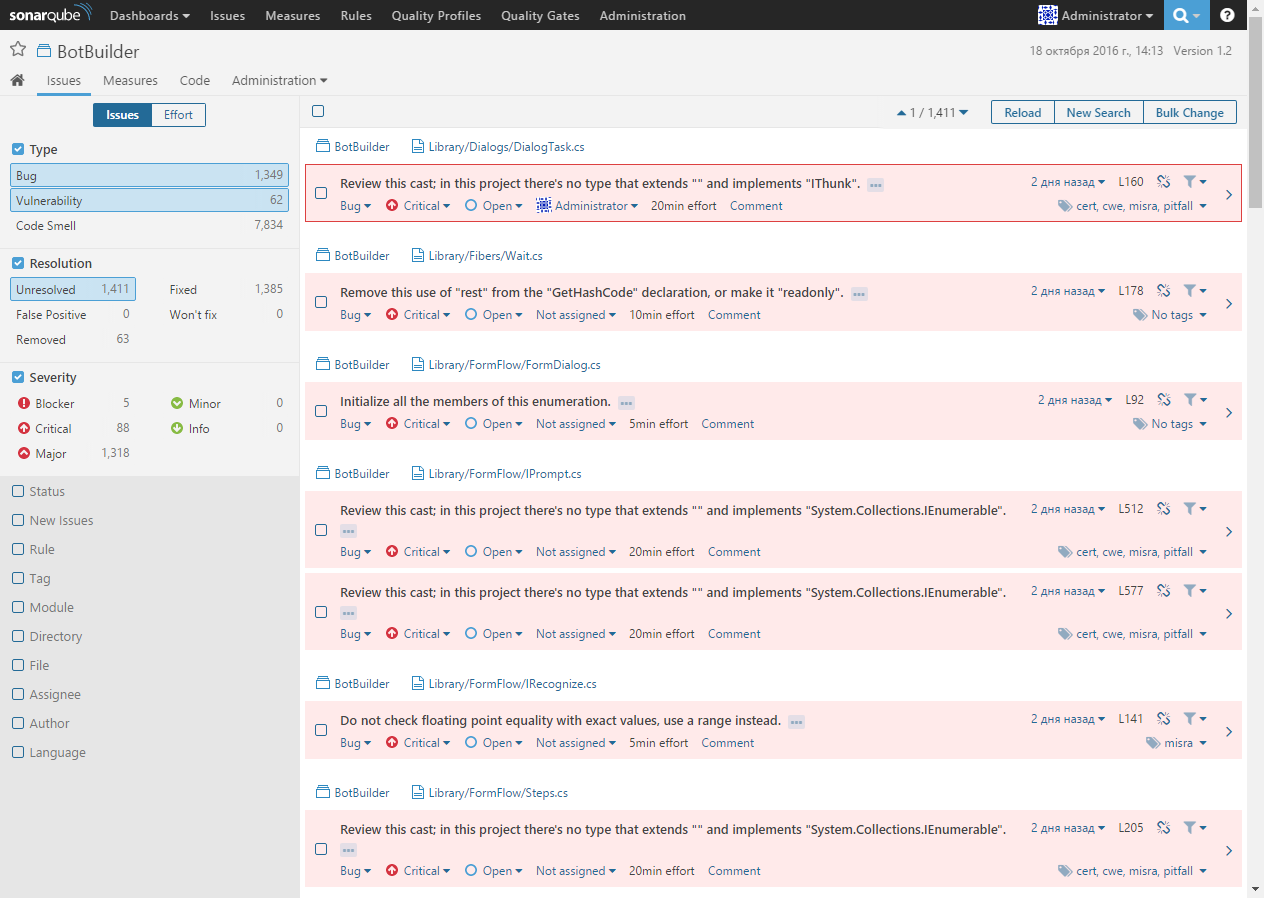
\includegraphics[height=8cm]{images/sonarQube.PNG}
  % The short caption should be capitalised
  % The full caption should hold a full sentence. 
 \caption[Anzeige von Fehlern und Problemen eines Projekts im SonarQube]{Anzeige von Fehlern und Problemen eines Projekts im SonarQube.}
  \label{fig:sonarQube}
\end{figure}

\subsection{Veracode}
Vercode ist eine Software-Lösung, die den Code auf Security-Lags und anderen Problemen untersucht. Diese Security-Lags Überprüfungen beinhalten unter anderem Open-Source und Third-Party-Tools, fehlerhafte Serverkonfigurationen, Cross-Site Scripting und mangelnde Validierungen. ~\parencite{veracodeSecurity}  Auch wird eine \textit{Software Composition Analysis} durchgeführt. Hierbei werden eingesetzte Open Source Tools auf Sicherheitslücken untersucht. Um eine Veracode-Analyse durchführen zu können, wird der Code auf eine bereitgestellte Website hochgeladen und dort automatisch analysiert und untersucht. Die Ergebnisse sind auf der Website einsehbar. Veracode arbeitet wie SonarQube mit dynamischen und statischen Tests, kann aber auch in Entwicklungsumgebungen eingebunden werden. Ebenso werden eine Vielzahl an Programmiersprachen unterstützt.  ~\parencite{veracodeDig}  

\section{Statische Code Analyse}
Die Code Analyse ist die Analysemöglichkeit des Quellcodes auf Fehler. Dazu ist Statische Code Analyse ist die Analysemöglichkeit des Quellcodes zur Übersetzungszeit. In dieser Analyse werden Prüfungen durchgeführt, die bestimmte Fehler, Regeln und Attribute identifizieren und aufzeigen. ~\parencite{gomes2009overview}
Die Statische Code Analyse soll ein gute Code-Qualität sicherstellen. Für die Beschreibung einer guten Code-Quality gibt es mehrere Modelle, wie das McCall Model, Boehm Model oder das ISO/IEC Proposed Model. ~\parencite{al2011software} Diese Modelle definieren bestimmte Faktoren, die für eine gute Code-Qualität wichtig sind: Portabilität, Interoperabilität, Korrektheit, Zuverlässigkeit, Effizienz, Integrität, Benutzerfreundlichkeit, Testbarkeit, Flexibilität und Wartbarkeit. \parencite{iqbalCodeQualityApproach} Diese Faktoren werden von allen Modellen als bestimmend hervorgehoben, die Modelle unterscheiden sich aber untereinander, wie zum Beispiel bei den Faktoren Dokumentation, Wiederverwendbarkeit und Möglichkeit zur Veränderung des Codes. ~\parencite{boukouchiModels}
Eine gute Code-Qualität kann aber nie durch Tools alleine sichergestellt werden, sondern es erfordert auch manuelle das Testen der Software. 

Die Analysetypen kann man in vier Arten unterteilen:
\begin{itemize}
\item \textbf{Syntaxanalyse}
Bei der Syntaxanalyse werden Fehler gefunden, ohne das der Code vollständig ausgeführt wird. Die Fehler sind daher reine Text-Fehler. Diese Fehler werden aber schon von Compiler und Interpreter gefunden.
\item \textbf{Stilanalyse}
In der Stilanalyse wird der Stil des Codes anhand bestimmter Regeln überprüft.
\item \textbf{Kontrolflussanalyse}
Hierbei wird der Ablauf des Programms analysiert.
\item \textbf{Datenflussanalyse}
In der Datenflussanalyse wird der Verlauf und der Wert einzelner Variablen des Programms analysiert.
\end{itemize}

\subsection{Unterschiede zu dynamischen Tests}
Im Gegensatz zur Statische Code Analyse überprüft die dynamische Code Analyse dynamischen und variablen Aspekte des Programms. Mit verschiedenen Eingabeparametern wird auf ein bestimmtes Ergebnis getestet. \cite{grigorenkoDynTest} Für diese Tests wird eine Simulation erstellt bzw. gestartet. Aus diesem Grund benötigt ein dynamischer Test ein lauffähiges Programm, was bei einem statischen Test nicht vorausgesetzt wird. Ein dynamischer Test auf zwei verschiedene Arten durchgeführt werden: Als Black-Box, White-Box oder diversifizierender Test.
In der Methode des Black-Box-Testings ist das zu testende System der Testerin oder dem Tester nicht bekannt. Hierbei wird ausschließlich die Funktionalität anhand der Spezifikationen getestet. Bei White-Box-Tests ist das System und der Code bekannt, daher sind die ausführenden Tester oft Entwicklerinnen und Entwickler des Programms. Anhand des Programms werden daher Tests erstellt, die bestimmte Teile überprüfen und testen sollen. Bei diversifizierenden Tests hingegen, werden die Testergebnisse nicht mit der Spezifikation verglichen, sondern sie vergleichen verschiedene Versionen der Software. Sind die getesteten Version gleich, so ist der Testfall erfolgreich. Ein diversifizierenden Test kann entweder als Back-to-back-Test (Testen von verschiedene Lösungen und Versionen des Programms), Regressionstest (Wiederholen des selben Tests um sicherzustellen, dass bereits getestete Software-Teile keine neuen Fehler aufweisen) oder als Mutationtest (Leistungsfähigkeit der Testmethoden) durchgeführt werden. \parencite{bommer2016softwarewartung}
\\
Um eine hohe Qualität des Programms zu gewährleisten, müssen daher beide Testverfahren kontinuierlich betrieben werden.
\section{Tools für die Statische Code Analyse}
Für die Statische Code Analyse gibt es eine Vielzahl an Anwendungen und Programmen. Diese Tools können Programmiersprachen-abhängig sein, es gibt aber auch Sprachen übergreifende Lösungen. Die Tools können für allgemeine Code-Smells, aber auch Lösungen für bestimmte Einsatzgebiete sein. Die Entwickler und Entwicklerinnen müssen für  spezifische Probleme und Faktoren bestimmte Tools einsetzten:

\begin{itemize}
\item \textbf{Code-Qualität} beschreibt, ob das Programm seine Funktionen richtig und effizient ausführt. Aber auch Leerzeichen und die Länge von Methoden und Klassen fallen in diese Kategorie. Tools für diese Einsatzbereiche sind CheckStyle oder FindBugs. Aber auch der Faktor der Wiederverwendbarkeit (Hinzufügen von neuen Features, Verwendbarkeit des Codes für andere Entwicklerinnen und Entwickler) fällt in diese Kategorie. Die Tools Jalopy und Crap4j testen den Code auf die Möglichkeit der Wiederverwendbarkeit. Dazu werden Analysen über den Testaufwand und Einhaltung der Coding-Richtlinien erstellt.
\item  \textbf{Code-Smells}
Ein Code-Smell (Bad-Smell) ist kein Compiler-Error oder Programmfehler. Als Code-Smells werden Codeteile bezeichnet, welche überarbeitet werden müssen. Auch das Design-Konzept kann als Bad-Smell bezeichnet werden. Beispiele von Code-Smells sind: Long Method, Temporary Field, Feature Envy, Complex Method und Duplicated Code. Werden Code-Smells nicht überarbeitet, kann es zu Strukturproblemen oder zu Problemen beim Refectoring kommen. Auch die Wiederverwendbarkeit des Codes wird dadurch beeinträchtigt. Code-Smells können durch Tools wie Checkstyle oder PMD identifiziert werden. \cite{palomba2014they}
\item \textbf{Nebenläufigkeit}
beschreibt die Möglichkeit, mehrere Funktionen zur selben Zeit auszuführen. Tools wie Sonar oder CheckThread untersuchen den Code hierbei auf Probleme, wie zum Beispiel Probleme beim Thread-Handling (siehe Race Conditions). Auch doppelter Code, der mit Nebenläufigkeit entfernt werden kann, wird angezeigt.
\item \textbf{Abhängigkeiten}
Beschreibt die Abhängigkeit eines Software-Moduls zu einem anderen Modul. In einer Programm sollten wenige Abhängigkeiten auftreten, da diese bei Ausfall Fehler oder Verzögerungen hervorrufen. Um Abhängigkeitsfehler wie Zirkelbezug vorzubeugen, können Tools wie JDepend oder Dependecy Finder eingesetzt werden. Unter Zirkelbezug versteht man das Auftreten einer Schleife bei Abhängigkeiten.
\item \textbf{Exception-Handling} Mit Exception-Handling können Software-Fehler für weitere Operationen aufgenommen und weitergegeben werden. Hierbei können Fehler wie Deadlocks, redundante Exception-Blocks und Null-Pointer auftreten. Um solche Fehler zu identifizieren können Tools wie JLint eingesetzt werden
\item \textbf{Kompatibilität} Darunter versteht man die Kompatibilität unter verschiedenen Versionen, unter auch zwischen Source- und Binary Code.  Clirr ist ein Tool das die Kompatibilität bei unterschiedlichen Java-Versionen untersucht. 
\item \textbf{Code-Style} Unter Style werden bestimmte Regeln und Coding-Conventions verstanden. Unter anderem gehören dazu Bestimmungen zu Leerzeichen, Klammern und Namenskonventionen. Für die Überprüfung des Code-Styles können Tools wie CheckStyle oder PMD eingesetzt werden.
\item \textbf{Speicherlecks}
Bei einem Speicherleck (memory leak) sind Daten im Arbeitsspeicher gespeichert,  welche aber nicht verwendet oder gelöscht werden. Tools wie Valgrind und Coverity können das Entstehen von Speicherlecks verhindern, indem sie mögliche Fehlerquellen wie Pointer oder Speicherzuweisungen untersuchen.
\item \textbf{Race Conditions}
Bei einer Race Condition greifen zwei verschiedene Services auf eine Ressource oder Methode zu. Da zwei Services nicht gleichzeitig die  gleiche Ressource verwenden können, kann nur eine der beiden Services auf das Ziel zugreifen. Das andere Service kann die Ressource nicht verwenden, was zu einem Fehler oder einem unerwünschten Ergebnis führen kann. Dieses Problem kann bei Threads auftreten. Tools wie JLint oder ConTest können ein Race Condition-Problem feststellen.
\item \textbf{Security}
Security ist ein wichtiger Punkt in Programmen. Tools wie FindBugs, Protecode und Xanitizer analysieren den Code und können Sicherheitsprobleme aufdecken, beispielsweise hard coded Passwörter, (Command) Injection und Response Splitting. \cite{goseva2015capability} Eine hierbei verwendete Technik ist die Taint-Analyse, wo der Datenfluss einer Dateneingaben überprüft wird. \cite{jung2014sensitive}
\end{itemize}

Um die einzelnen Tools bewerten und vergleichen zu können, müssen sie daher in verschiedene Anwendungsbereiche geteilt werden. Bei einer Bewertung der Tools sind aber auch andere Metriken ausschlaggebend wie: Möglichkeit der Erweiterbarkeit der Tools (Open-Source), letztes Release und Art und Vielfalt der Reports. ~\parencite{comparativeAnalysisTools}

\section{Visualisierungen} 
In den vorgestellten Lösungen gibt es mehrere Arten die Analyseergebnisse einsehen zu können:
\begin{itemize}
\item \textbf{Anzeige in der Entwicklungsumgebung}
\item \textbf{Anzeigen in eigenen Desktop-Applikation}
\item \textbf{Anzeige in Webbrowsern}
Besonders bei der Integration der Statischen Code Analyse in Build-Servern.
\item \textbf{Anzeige als Report: XML oder HTML (siehe Abbildung \ref{fig:checkstyleHTMLReport}}
\begin{figure}[tp]
  \centering
  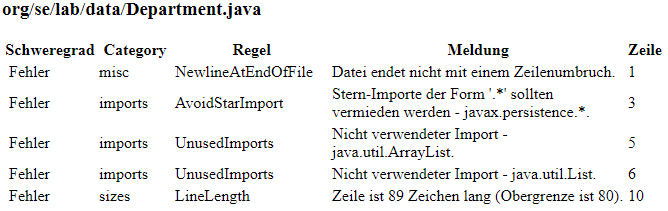
\includegraphics[height=5cm]{images/checkstyleHTMLReport.PNG}
  % The short caption should be capitalised
  % The full caption should hold a full sentence. 
 \caption[Auszug aus dem automatisch generierten CheckStyle-Report der Ergebnisse der Analyse. (vgl. Abbildung in der Entwicklungsumgebung \ref{fig:findingsInIDE})]{Auszug aus dem automatisch generierten CheckStyle-Report der Ergebnisse der Analyse. (vgl. Abbildung in der Entwicklungsumgebung \ref{fig:findingsInIDE})}
  \label{fig:checkstyleHTMLReport}
\end{figure}
\end{itemize}
\subsection{Probleme} 

\subsubsection{Keine dauerhafte Anzeige} 
Der Fokus der Ergebnisanzeige der Statischen Code Analyse in Entwicklungsumgebungen liegt auf das Ausbessern der gefunden Fehler. Die Fehler und Informationen werden daher nach der Ausbesserung nicht mehr angezeigt. Die Entwicklerin oder der Entwickler kann die ausgebesserten Fehler nicht mehr einsehen.

\subsubsection{Keine Verbesserung der Kenntnisse und des Codestils des Entwicklers} 
Da die Fehler nicht dauerhaft angezeigt werden, kommt es zu keiner Verbesserung der Programmierkenntnisse der Entwickler und Entwicklerinnen. Weiters kann in Entwicklungsumgebungen die automatische Ausbesserung getätigt werden, sodass der Entwickler oder die Entwicklerin oft den Fehler nicht bewusst überdenken und selber ausbessern wird. 
Die selben Fehler häufen sich daher immer wieder. Dies geschieht auch, weil besonders unerfahrenere Entwickler einige Fehlerwarnung nicht nachvollziehen und verstehen können, da es keine Möglichkeit gibt die Bugs genauer einsehen zu können. 

\subsubsection{Unübersichtliche Anzeige} 
In großen Klassen, wo sich viele Fehler und Informationen befinden, gehen die einzelnen Fehler in der kleinen Übersichtsanzeige oft unter. In der Zeile, wo sich der Fehler befindet, kann der Fehler nur mit einem Mouseover über die Warnung angezeigt werden. 

\subsubsection{Keine weiteren Analysen}
Weitere Informationen wie Zusammenhänge der Fehler, Analyse der Fehlerquellen, Häufigkeitsverteilungen und zeitliche Veränderungen werden nicht angezeigt. So gehen wichtige Informationen für den Entwickler verloren.        % research related (to your!) work 
%%%%%%%%%%%%%%%%%%%%%%%%%%%%%%%%%%%%%%%%%%%%%%%%%%%%%%%%%%%%%%%%%%%%%%%%%%%%%
\chapter{Konzept}
\label{chap:concept}
%%%%%%%%%%%%%%%%%%%%%%%%%%%%%%%%%%%%%%%%%%%%%%%%%%%%%%%%%%%%%%%%%%%%%%%%%%%%%
\chapterstart
Um die beschriebenen Problemstellungen zu lösen und diese Ergebnisse auch evaluieren zu können, wird eine Applikation entwickelt. In dieser Applikation werden die Ergebnisse der Statischen Code Analyse aufbereitet, visualisiert und angezeigt. Die Daten müssen für die Möglichkeit einer langfristigen Auswertung dauerhaft in einer Datenbank gespeichert werden. \\\\ Für die Testdaten werden gezielt Tools in verschiedenen Projekten eingesetzt. Die Daten werden in die Datenbank importiert. 
\begin{figure}[tp]
  \centering
  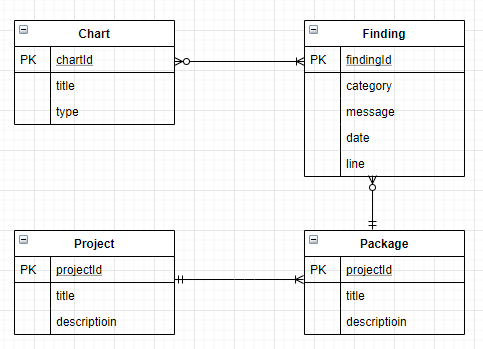
\includegraphics[height=6cm]{images/chartERD.PNG}
  % The short caption should be capitalised
  % The full caption should hold a full sentence. 
 \caption[Beispiel-ERD, mit der die Daten für die weitere Aufbereitung gespeichert werden können.]{Beispiel-ERD, mit der die Daten für die weitere Aufbereitung gespeichert werden können.}
  \label{fig:chartERD}
\end{figure}
Um die Daten in die Datenbank importieren zu können, ist eine zusätzliche Lösung erforderlich. Diese zusätzlich Lösung als Batch-Job, manueller Importer oder als Plugin erstellt werden. Da ein Batch-Job oder ein Importer eine zusätzliches Applikation erfordert, wird in Plugin implementiert. Dieses Plugin kann auch konfiguriert werden, damit der Entwickler oder die Entwicklerin die Datenquellen und den Zeitpunkt des Imports selber festlegen können. In der Abbildung \ref{fig:chartERD} wird eine Möglichkeit dargestellt, wie diese Daten in der Datenbank gespeichert werden können und so als Basis für die Visualisierungen und Tabellen dienen können. \\\\
In der der Applikation können die Benutzer und Benutzerinnen die Daten gezielt auslesen. Da die Daten eine große Menge an Daten über einen großen Zeitraum gespeichert werden sollen, ist eine Filterung der Daten notwendig. Die Visualisierungen in der Applikation betreffen die Fehler und versuchen Fragen zu lösen wie: Wo sind die meisten Fehler aufgetreten? Was sind die häufigsten Fehler und wie kann man die Fehler vermeiden? Welche packages erfordern ein Refactoring? Diese Fragen sollen in Charts beantwortet werden, die mit den Daten automatische generiert werden. Die Applikation ist daher für den einzelnen Entwickler, als auch für das ganze Entwicklungs-Team von Interesse. Diese Informationen sollen auch als Information versendet oder gespeichert werden können, daher soll ein Export der Daten möglich sein. Der Export wir als PDF-Dokument generiert, da so alle Daten formatiert und gelistet ausgegeben werden können. \\\\ Die Applikation wird als Webapplikation entwickelt. Dies bietet den Vorteil, dass die Daten und mögliche Einstellungen und Konfigurationen für alle Entwicklerinnen und Entwickler verfügbar sind und die Webapplikation zentral für alle verfügbar ist. Ein Nachteil, gegenüber einer Desktopapplikation oder einer Extension für die Entwicklungsumgebung ist hierbei die fehlende Möglichkeit, direkt und automatisch zu den Fehlerquellen zu navigieren. Der Fokus der Webapplikation richtet sich aber auf die Übersicht, Visualisierung und die kontinuierliche Verbesserung des Codes der Benutzerinnen und Benutzer. \\\\ Die Visualisierungen sollen so erstellt werden, das sie unabhängig der eingesetzten Tools erstellt werden können. Die Visualisierungen sollen modern und einfach verständlich präsentiert werden.


%Your text here\ldots
%Describe an overall concept of a solution, which could possibly solve a given problem. Design a novel solution and visualise the architecture and relevant (data) flows. Compare and relate your approach to possible alternatives and argue why the suggested solution will be better. woher testdaten; wie vorgehn bei entwicklung; was soll gelöst werden; was soll noch kommen;

\chapterend        % concept/design of solution

\chapter{Umsetzung}
\section{Technologien und Tools für Umsetzung } 

\subsubsection{Java} 
Die drei Teilprojekte der Arbeit wurden in Java entwickelt. Die verwendete Java Version ist Java 11. 

\subsubsection{Spring} 
Spring Boot ist ein Java Framework, das im Zuge der Projektarbeit zur Entwicklung der Web-Applikation verwendet wurde.

\subsubsection{Maven} 
Maven ist ein Versionsverwaltungstool mit dem Abhängigkeiten und JARs verwaltet und heruntergeladen werden können.

\subsubsection{FindBugs/SpotBugs} 
ERGÄNZEN ERGÄNZEN ERGÄNZEN 

\subsubsection{Checkstyle} 
Checkstyle ist ein open-source Tool für die Statische Code Analyse. Checkstyle ist für die Verwendung in Java Applikation entwickelt worden. Hierbei werden eine Vielzahl an Fehler und Bugs analysiert und beachtet. Checkstyle kann konfiguriert und an spezifische Probleme angepasst werden

\subsubsection{MongoDB} 
Als Datenbank wird MongoDB verwendet. Es ist ein nicht-relationales Datenbankmanagementsystem. Es gehört zu den dokumentorientierten Datenbanken.
MongoDB kann über die offiziele Website heruntergeladen und installiert werden. Um MongoDB zu starten, muss im \textit{/bin} Folder der Befehl \textit{mongo} ausgeführt werden.
\cite{mongoDbManual}

\subsubsection{MongoDB Java Driver}
Der MongoDB Java Driver wird für die Kommunikation (Synchronisation und asynchrone Interaktion) mit MongoDB eingesetzt. Als Alternative kann Jongo (https://jongo.org/) oder  Morphia (https://morphia.dev/) eingesetzt werden. 

\subsubsection{JavaScript und Frameworks}
Für das Frontend der Webapplikation wird JavaScript eingesetzt. Um zusätzliche Funktionen verwenden zu können, werden folgende JavaScript-Plugins, Frameworks und Libraries verwendet: 
\begin{itemize}
\item JQuery 
\item Bootstrap
\item DataTables \\ Bietet automatische Pagination und Sortierfunktionen für Tabellen 
\item Chart.js \\ Unterstützt das Erstellen von Diagrammen. 
\end{itemize}

\subsubsection{IntelliJ}
IntelliJ IDEA wurde als Entwicklungsumgebung für das Backend und Frontend verwendet. 

\section{Infrastruktur und Aufbau der Applikationen} 
Im Rahmen dieser Arbeit wurde mehrere Applikationen und Systeme verwendet. Die Arbeit setzt sich aus folgenden Teilen zusammen:

\begin{figure}[tp]
  \centering
  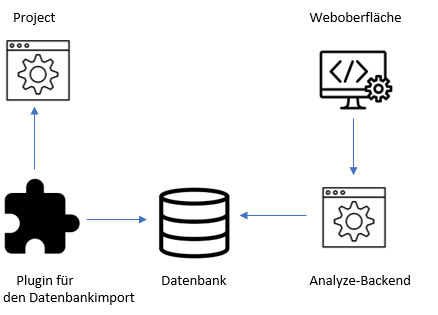
\includegraphics[height=8cm]{images/infrastruktur.PNG}
  % The short caption should be capitalised
  % The full caption should hold a full sentence. 
 \caption[Aufbau der Teilsysteme und Projekte der Arbeit]{Aufbau der Teilsysteme und Projekte der Arbeit.}
  \label{fig:engine}
\end{figure}

Das \textit{Project} ist das Softwareprojekt, welches analysiert werden soll. In diesem Projekt wird auch ein Tool für die Statische Code Analyse eingesetzt. Dieses Tool speichert die Daten (Errors, Warnungen, Informationen) extern. Um diese Daten für die Analyse verwenden zu können, wurde im Rahmen der Arbeit ein \textit{Plugin}, welches das Projekt einsetzten kann, entwickelt. Dieses Plugin greift auf die Daten Statische Code Analyse zu. der Um das Plugin verwenden zu können, muss auch eine \textit{Datenbank} angegeben werden, in welche das Plugin die Daten der Statische Code Analyse des Projekts speichern kann. Die nicht-relationale Datenbank wird auf einem Server gehostet. Um in der Weboberfläche die Daten der Datenbank anzeigen zu können, wird auch ein \textit{Backend} benötigt. Das Backend liest die Daten aus und gibt sie an die Weboberfläche weiter. In der \textit{Weboberfläche} werden die Daten in verschiedenen Diagrammen und Tabellen ausgewertet. Auch ein PDF-Export ist möglich. 


\section{Demo-Projekt und Bugreport}
demo projekte allgemein -> unterschiedlichkeit
%https://checkstyle.sourceforge.io/config_filters.html

\subsection{Entwicklungsumgebung Build-in}
eingehen auf verwendete ide und tools; intellij inspection build in 
https://www.jetbrains.com/help/idea/code-inspection.html

\subsection{Maven Plugins}
Viele Tools für die Statische Code Analyse bieten die Möglichkeit, XML-Reports zu genieren. Dies ist möglich mit dem Verwenden der spezifischen Maven-Plugins. \cite{spotBugsUsage} \cite{checkstylePlugin} 
Diese Plugins bieten build-Optionen an, mit dem die XML oder Doc-Reports generiert werden können.
\subsubsection{CheckStyle-Plugin}
Um Checkstyle verwenden zu können, muss das CheckStyle-Plugin nicht verwendet werden. Das Plugin dient zum Export der Daten als XML. Dieses generierte XML bildet den Grundstock für die unterschiedlichen Präsentationen der Daten im Frontend gibt. Um die Daten zu exportieren muss folgender Befehl ausgeführt werden:
\begin{verbatim}
mvn checkstyle:checkstyle
\end{verbatim}
Dieser Befehl muss von der Benutzerin oder dem Benutzer manuell ausgeführt werden. Um den Report automatisch zu erstellen, kann beim Einbinden des Plugin die Phase angegeben werden:

\lstset{
  caption={Das Plugin wird automatisch in der install-Phase ausgeführt.}, 
  basicstyle=\small\ttfamily, 
  label=lst:main, 
  %float=tbhp, % float image to top/bottom/here/page
  language=Java,
  frame=single,
  breaklines=true, % break long source code lines, and add arrow
  postbreak=\mbox{\textcolor{red}{$\hookrightarrow$}\space},
  %  basewidth={0.55em}, 
  % fontadjust}  % adjust these for more appealing appearance
}

% listing with some settings, such as float, for this listing only
\begin{samepage}% with samepage we keep a FLOATing listing on one page
	\begin{lstlisting}[float=tbhp]
<plugin>
  <groupId>org.apache.maven.plugins</groupId>
  <artifactId>maven-checkstyle-plugin</artifactId>
  <version>3.1.1</version>
  <executions>
    <execution>
      <phase>install</phase>
      <goals>
        <goal>checkstyle</goal>
      </goals>
    </execution>
  </executions>
</plugin>
	\end{lstlisting}
\end{samepage}

Das generierte XML-File wird im /target Ordner abgelegt.
\subsubsection{SpotBugs-Plugin}
ERGÄNZEN TESTEN
\begin{verbatim}
mvn site
\end{verbatim}
Der Speicherort des generierten XML-Files kann in der Plugin-Konfiguration angegeben werden.


\section{Speichern der Daten} 

Zum Speichern der Daten wird eine Datenbank benötigt. Aufgrund der stark variierenden Daten und da es bei großen Projekten auf einem längeren Zeitraum viele Fehler und Warnungen gefunden werden, wird eine nicht-relationale Datenbank (NoSQL) verwendet. 

\subsection{Vorteil vom Einsatz einer nicht-relationalen Datenbank gegenüber einer relationalen Datenbanke }
Der Vorteil einer nicht-relationalen Datenbank wie MongoDB besteht in der unterschiedlichen Lösung des CAP-Theorem. CAP ist eine für Abkürzung:

\begin{itemize}
\item C = Consistency (Konsistenz)
\item A = Abailability (Verfügbarkeit) 
\item P = Partition Tolerance (Fehlertoleranz))
\end{itemize}

Das CAP-Theorem besagt, dass nur zwei dieser Eigenschaften gleichzeitig gelten können. 
Relationale Datenbanken sind im CA Bereich beheimatet, sie legen einen hohen Wert auf Konsistenz. Bei NoSQL und Big Data muss  auf die Fehlertoleranz geachten werden und gleicherweise müssen die Datenbanken hochverfügbar sein, so sind sie im AP Bereich beheimatet. Das garantiert eine hohe Verfügbarkeit und Fehlertoleranz. Konsistenz ist bei den vielen Analysen der Statischen Code Analyse weniger von nutzen, da die Daten der verschiedenen Tools auch stark varrieren. Zusätzlich garantiert die Verwendung einer nicht-relationalen Datenbank eine einfache Query-Language und ein freies Schema.\\
Die Verwendung von nicht-relationalen Datenbanken stellt daher eine Möglichkeit da, die Herausforderungen im Bereich von BigData zu lösen:
\begin{itemize}
\item Größe der Daten (Volume) 
\item Geschwindigkeit der Verarbeitung (Velocity)
\item Strukturierung der Daten (Variety)
\end{itemize}


\subsection{Typen der nicht-relationale Datenbanken}
NoSQL bedeutet nicht \emph{Kein SQL}, sondern \emph{Not only SQL}. Der Aufbau ist hierbei nicht auf relationale Datenbanken beschränkt, sondern kann seine Datenbankstruktur erweitert. 
So gibt es in diesem Umfeld viele Anbieter von NoSQL Lösungen. Diese Lösungen für Datenbanken werden in folgende Kategorien unterteilt:

\begin{itemize}
\item Key Value Datenbanken: Abfragen nur über einen Schlüssel
\item Spaltenorientierte Datenbanken (Dynamische Spalten)
\item Graph-Datenbanken (Verwaltung und Arbeiten mit Knoten)
\item Dokumentorientierte Datenbanken: Besteht aus mehreren Dokumenten (JSONs)
\end{itemize}

Da die Analyseergebnisse der Statischen Code Analyse mehrere Informationen beinhalten, die leicht in JSONs gespeichert werden können, wird die dokumentorientierte Datenbank MongoDB verwendet. 

\subsection{Aufbau der Datenbank}
MongoDB benutzt schemafreie Collections um Daten zu speichern. Schemafreiheit ist nur ein technischer Aspekt. Eine Collection kann Dokumente mit beliebiger Struktur speichern und jedes dieser Dokumente kann sich von den anderen Dokumenten unterscheiden. Trotzdem sollen nicht stark unterschiedliche Dokumente in einer Collection gespeichert werden, da es in der Verwaltung bei einer starken Abweichung einen großen zusätzlichen Aufwand gibt. 

Für die Analyseergbnisse wird eine Collection verwendet, die folgende Felder beinhalten kann: \textit{id, project, file, line, message, source, severity, date}

Beispiel eines JSON-Datensatzs in der Collection:

\begin{verbatim}
{ "_id" : ObjectId("5e1209881a2dff20ab6ee6c6"), 
"project" : "importerProject", 
"file" : "Sender.java", 
"line" : 72, 
"message" : "Not closed!", 
"source" : "checkstyle.checks.blocks.AvoidNestedBlocksCheck", 
"severity" : "error", 
"date" : ISODate("2020-01-05T00:00:00Z") }
\end{verbatim}

In einer relationalen Datenbanken mit einem starken Schema und einer ausgeprägten Konsistenz, könnte dieser Datensatz in mehrere Tabellen verteilt gespeichert werden, zum Beispiel eine eigene Tabelle für \textit{severity}. Aufgrund der schwachen Konsistenz in nicht-relationalen Datenbanken wird hierbei nur eine Collection (Tabelle) verwendet. So können in dieser Collection auch Datensätze gespeichert werden, die keine \textit{severity} besitzen: NULL-Werte können so nicht auftreten. \\
Die Datensätze können mit dem Mongo-Service ausgelesen werden: 

\begin{verbatim}
// Lesen aller Daten:
db.findings.find({})

// Lesen eines bestimmten Datensatzes:
db.findings.find({"_id" : ObjectId("5e1209881a2dff20ab6ee6c6")})
\end{verbatim}

Eine zweite Collection \textit{recommendations} wird für das Speichern der Vorschläge für die Fehler und Warnungen verwendet. Benutzer können hierbei über die Webapplikation Tutorials und nützliche Links zu den einzelnen Fehlern und Warnungen speichern.
In dieser Collection werden daher Objekte mit nur zwei Datenfeldern gespeichert: \textit{error} und \textit{link}. \\
In einer dritten Collection \textit{ignoredFindings} werden Errors und Warnungen gespeichert, die von der Anzeige im Frontend ausgenommen werden. In den Objekten gibt es nur ein Datenfeld \textit{message}, für die ausgenommen Meldungen.
\section{Datenbank Importer Plugin} 
Die Statischen Code Analyse wird auf dem Rechner des Entwicklers oder der Entwicklerin ausgeführt. Diese Daten müssen in der Datenbank gespeichert werden, um sie in einem längeren Zeitraum einsehen und auswerten zu können. Eine eigene Lösung wird daher benötigt, um die Daten in der Datenbank speichern zu können. 
\subsection{Apache Maven Plugin}
Mit Apache Maven können verschiedene Plugins eingebunden und im Projekt verwendet werden. Apache Maven bietet aber auch die Möglichkeit, eigene Plugins zu entwickeln.\cite{anardu2014maven}

Die Dependency \textit{maven-plugin-api} gibt Klassen und Funktionen vor, die benutzt werden können um ein eigenes Plugin zu entwickeln
\begin{verbatim}
 <dependency>
      <groupId>org.apache.maven</groupId>
      <artifactId>maven-plugin-api</artifactId>
      <version>3.6.0</version>
      <scope>provided</scope>
 </dependency>
\end{verbatim}

Mit dieser Dependency kann nun eine Mojo-Klasse erstellt. (\textit{MainExecuter.java}) Sie stellt den Kern des Plugins da, die der Verwendung des Plugins zuerst ausgeführt wird. \cite{gonzalezMavenTutorial}

\lstset{
  caption={Kopf der Executor-Klasse: Sie wird mit dem Aufruf des Plugins zuerst gestartet.}, 
  basicstyle=\small\ttfamily, 
  label=lst:main, 
  %float=tbhp, % float image to top/bottom/here/page
  language=Java,
  frame=single,
  breaklines=true, % break long source code lines, and add arrow
  postbreak=\mbox{\textcolor{red}{$\hookrightarrow$}\space},
  %  basewidth={0.55em}, 
  % fontadjust}  % adjust these for more appealing appearance
}

% listing with some settings, such as float, for this listing only
\begin{samepage}% with samepage we keep a FLOATing listing on one page
	\begin{lstlisting}[float=tbhp]
@Mojo(name = "import", defaultPhase = LifecyclePhase.INSTALL)
public class MainExecutor extends AbstractMojo {

    @Parameter(property = "dbName",defaultValue = "findings")
    private String dbName;
	\end{lstlisting}
\end{samepage}
	

Um die Klasse \textit{MainExecuter.java} als Mojo-Klasse zu kennzeichen, muss von \textit{AbstractMojo} abgeleitet und mit \textit{@Mojo} annotiert werden.

%\includegraphics{/dbpluginConnect.PNG}

Mit der Option \textit{defaultPhase} kann festgelegt werden, in welcher Maven-Lifecycle-Phase das Plugin ausgeführt werden soll. Mit dieser Einstellung wird das Plugin während des install-Prozesses ausgeführt. Weitere Möglichkeiten sind unter anderen die Phasen  \textit{deploy},  \textit{clean} und  \textit{compile}. \\

Das Plugin wird mit bestimmten Parametern aufgerufen. Diese können beim Einbinden des Plugins angegeben werden. Folgende Parameter werden benötigt, um das Plugin auszuführen:

\begin{itemize}
\item \textit{dbName}: Name der Datenbank, indem die Ergebnisse der Statischen Code Analyse gespeichert werden. 
\item \textit{dbUrl}: URL für die Datenbank
\item \textit{xmlFile}: Name des generierten XML-Files
\end{itemize}
  
% \includegraphics{dbpluginParameter}    

In der Mojo-Klasse muss die Methode \textit{execute} implementiert werden, die zu Beginn, beim Start des Plugins, ausgeführt wird. Mithilfe der oben definierten Parameter und des Projektnamens, der mit dem Maven-Lifecycle ausgelesen werden kann, wird nun der Import in die Datenbank gestartet. 

\subsection{MongoDB-Java-Driver und Datenbank-Import}
Der Importer speichert die Daten des XML-Reports in Datenbanken. Dazu wird das XML-File ausgelesen und die einzelnen gefundenen Fehler und Informationen werden in Java-Objekte umgewandelt. Das Speichern der Java-Objekte in den Collections ist ohne Konvertierung, im Vergleich zu anderen herkömmlichen Tools wie Hibernate, nicht möglich. Um Daten zu speichern, müssen die Java-Objekte in Dokumente umgewandelt werden. Daher muss ein Konverter implementiert werden: \textit{DBObjectConverter}
Bei steigender Komplexität und Größe der Datenbank können die Konverter sehr komplex werden. Der Typ \textit{org.bson.Document} wird vom MongoDB-Java-Driver vorgegeben. Ein BSON-Dokument unterscheidet sich nur von der Kodierung zu Json-Objekte. (BSON=Binary Json) 
Diese Dokumente können nun für die Datenbank-Transaktionen verwendet werden. \\

Um die Dokumente speichern zu können, muss eine Verbindung zur Datenbank mit den eingegebenen Parametern erstellt werden. Dazu müssen Objekte mit den Typen \textit{MongoClient}, \textit{MongoDatabase} und \textit{MongoCollection} initialisiert und verwendet werden:

\lstset{
  caption={Benötigte Attribute, um sich mit der Datenbank verbinden und die Collections verwenden.}, 
  basicstyle=\small\ttfamily, 
  label=lst:main, 
  %float=tbhp, % float image to top/bottom/here/page
  language=Java,
  frame=single,
  breaklines=true, % break long source code lines, and add arrow
  postbreak=\mbox{\textcolor{red}{$\hookrightarrow$}\space},
  %  basewidth={0.55em}, 
  % fontadjust}  % adjust these for more appealing appearance
}

% listing with some settings, such as float, for this listing only
\begin{samepage}% with samepage we keep a FLOATing listing on one page
	\begin{lstlisting}[float=tbhp]
	
mongoClient = new MongoClient(new MongoClientURI(dbUrl));
db = mongoClient.getDatabase(databaseName);
db = mongoClient.getDatabase(databaseName);

	\end{lstlisting}
\end{samepage}

Der Typ \textit{MongoCollection<Document>} kann nun verwendet werden um Dokumente zu speichern, löschen oder auszulesen. Diese Operationen werden beim MongoDB-Java-Driver direkt auf die betreffenden Collections angewendet. Ein Commit oder eine andere Operation ist dabei nicht notwendig.

% \includegraphics{dbpluginSave}    

\section{Webapplikation} 
Die Webapplikation bildet den zentralen Teil der Applikation. Das Ziel ist es, die gespeicherten Daten für die Benutzerinnen und Benutzer übersichtlich und einfach aufzubereiten. 
\subsection{Backend}
Im Backend werden die Daten aus der Datenbank in Services ausgelesen. Die ausgelesen Daten werden in Beans umgewandelt. Über die REST-Schnittstelle können Daten an das Frontend übergeben werden. Das Backend bzw. die Webapplikation verwendet das Framework Spring-Boot als Alternative zu Java EE. \cite{walls2016spring} Spring Boot bietet einen Standalone-Server und kann daher ohne Konfigurationen verwendet werden. Zusätzlich bietet Spring Boot die Möglichkeit zur Erstellung von Spring Beans und REST-Controller.  

\subsubsection{Struktur}
aufbau der packages und files; image
\subsubsection{API und Controller}
Über den Controller können HTTP-Requests an das Backend geschickt werden. Mit Spring können die Controller als \textit{RestController} annotiert und verwendet werden. Die einzelnen Methoden des Controllers werden zusätzlich annotiert um die Methode (GET, POST, DELETE, PUT, ...) und den Pfad zu definieren. Im Pfad können zusätzlich Parameter als \textit{PathVariable} definiert werden. Im Controller werden  Methoden verwendet um bestimmte Projektanalysedaten auszulesen, Daten als PDF zu exportieren und um Vorschläge zu speichern und auszulesen. Im \textit{FindingsController} werden die Anfragen aus dem Frontend bearbeitet und Daten an des Frontend übermittelt. Im Controller sind dazu die verschiedenen Services eingebunden.
\subsubsection{Services und MongoDB-Java-Driver}
In den Services werden Methoden bereitgestellt, die die Daten der Datenbank auslesen. Dies geschieht mit dem MongoDB-Java-Driver. Für das Verwenden des MongoDB-Java-Driver ist ein spezifischer Converter notwendig. Das Mapping der Java-Objekte mit den Collections ist ohne konvertierung, im Vergleich zu Hibernate, nicht möglich. Um Daten zu speichern, müssen die Java-Objekte  in Dokumente umgewandelt werden und um ausgelesene Dokumente zu verwenden, müssen die Dokumente in Java Objekte umgewandelt werden. Daher muss ein Konverter verwendet werden: \textit{DBObjectConverter.java}
Bei steigender Komplexität und Größe der Datenbank werden auch die Konverter komplexer. 

\lstset{
  caption={Um die Datenbank benutzen können, müssen die Java-Objekte bzw. die Datenbank-JSON-Objekte konvertiert werden.}, 
  basicstyle=\small\ttfamily, 
  label=lst:main, 
  %float=tbhp, % float image to top/bottom/here/page
  language=Java,
  frame=single,
  breaklines=true, % break long source code lines, and add arrow
  postbreak=\mbox{\textcolor{red}{$\hookrightarrow$}\space},
  %  basewidth={0.55em}, 
  % fontadjust}  % adjust these for more appealing appearance
}

% listing with some settings, such as float, for this listing only
\begin{samepage}% with samepage we keep a FLOATing listing on one page
	\begin{lstlisting}[float=tbhp]
public static Finding convertToObject(Document e) {
    String project = (String) e.get("project");
    String file = (String) e.get("file");    
    ...

public static Document convertToDocument(Recommendation rec) {
    org.bson.Document recDoc = new Document();
    recDoc.append("error", rec.getError());
    recDoc.append("link", rec.getLink());
    ...
	\end{lstlisting}
\end{samepage}

Der Konverter wird in allen Service-Methoden verwendet, wo Daten aus den Collections mit dem MongoDB-Java-Driver ausgelesen, gespeichert oder gelöscht werden. Um diese Operation zu verwenden, müssen die Methoden \textit{find}, \textit{deleteOne} und \textit{insertOne} verwendet werden. Um bestimmte Daten auszuwählen, wird in der Methode \textit{find} ein Query-Parameter übergeben: In den entsprechenden Services ein Projektname oder ein Datum. Die Ergebnisse werden mit einem Iterator iteriert und an den Konverter übergeben. Eigene Services gibt es für alle Datenbank Collections: Findings, Recommendation, IgnoredMessages.

\subsubsection{IText und PDF-Export}
Der PDF-Export ist eine weitere Funktion, die das Backend bietet. Ein PDF-Export kann für ein bestimmtes Projekt in einem bestimmten Zeitraum erstellt werden. Im Report werden die wichtigsten Informationen der Analyse in Textform dargestellt, dazu auch die einzelnen gefundenen Fehler und Warnungen. \\
Dazu wird das Tool IText zur Erstellung von Reports verwendet.  \cite{lowagie2011itext} Um IText zu verwenden, kann aus verschiedenen Preismodellen gewählt werden, eine kostenlose Version wird aber auch zur Verfügung gestellt und in dieser Arbeit verwendet.  \\
Über das Service liest der PDF-Generator die angegeben Daten aus.

\lstset{
  caption={Initialisierung des Writers um im Dokument einen Paragraph zu erstellen.}, 
  basicstyle=\small\ttfamily, 
  label=lst:main, 
  %float=tbhp, % float image to top/bottom/here/page
  language=Java,
  frame=single,
  breaklines=true, % break long source code lines, and add arrow
  postbreak=\mbox{\textcolor{red}{$\hookrightarrow$}\space},
  %  basewidth={0.55em}, 
  % fontadjust}  % adjust these for more appealing appearance
}

% listing with some settings, such as float, for this listing only
\begin{samepage}% with samepage we keep a FLOATing listing on one page
	\begin{lstlisting}[float=tbhp]
PdfWriter writer = PdfWriter.getInstance(
   document, byteArrayOutputStream);
document.open();
document.add(new Paragraph(
  "Findings PDF Export. - " +LocalDate.now(), titleFont));

	\end{lstlisting}
\end{samepage}

Für alle im Service ausgelesen Daten wird ein eigener Paragraph(Zeile) erstellt. Um die Überschrift und die Daten entsprechend zu formatieren, kann mittels \textit{IText} auch ein Font erstellt werden. Mit der \textit{FontFactory} wird hierbei ein Font mit bestimmter Schriftart, Schriftgröße und Farbe erstellt.
Nach der Erstellung des PDF-Dokument muss das Ergebnis weiter an den Client geschickt werden. Um das PDF-Dokumente im \textit{Response} der HTTP-Anfrage zu übertragen, wird das Dokument in ein \textit{byte-array} konvertiert. Dies geschieht mit der Verwendung des \textit{ByteArrayOutputStream} und dessen Methode \textit{toByteArray}. 

\begin{figure}[tp]
  \centering
  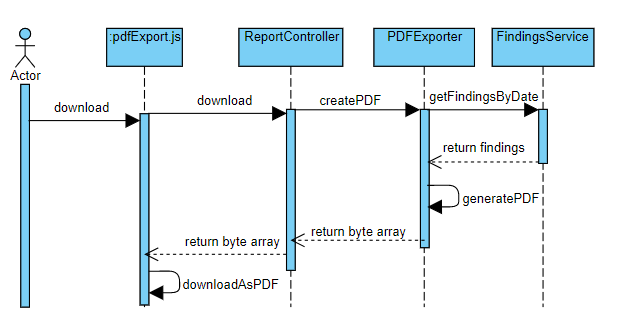
\includegraphics[height=8cm]{images/seqGeneratePdf.PNG}
  % The short caption should be capitalised
  % The full caption should hold a full sentence. 
 \caption[Sequenzdiagramm für den Download eines PDF-Exports]{Sequenzdiagramm für den Download eines PDF-Exports.}
  \label{fig:engine}
\end{figure}

\subsection{Frontend}
Im Frontend werden die Daten in verschiedenen Formen aufbereitet und den Entwicklerinnen und Entwicklern präsentiert, dazu dient eine OnePage-HTML Seite. Die Daten im Frontend werden aus dem Backend abgefragt.
\subsubsection{Struktur}
aufbau der ordner und files; image
\subsubsection{Kommunikation mit dem Backend}
Die Kommunikation zwischen Frontend und Backend geschieht mittels HTTP-Calls. Die im Frontend gesendeten HTTP-Calls werden im Backend-Controller verarbeitet.  Mit der JavaScript Schnittstelle \textit{XMLHttpRequest} werden HTTP-Methoden (POST, GET) abgeschickt. Ein Vorteil von \textit{XMLHttpRequest} ist die Möglichkeit der Asynchronen-Ausführung der Requests. Daher können auch dynamische Daten abgerufen werden.  \cite{ajaxOnJava}
\lstset{
  caption={Erstellung eines GET-Request für Projektdaten mit der Schnittstelle XMLHttpRequest.}, 
  basicstyle=\small\ttfamily, 
  label=lst:main, 
  %float=tbhp, % float image to top/bottom/here/page
  language=Java,
  frame=single,
  breaklines=true, % break long source code lines, and add arrow
  postbreak=\mbox{\textcolor{red}{$\hookrightarrow$}\space},
  %  basewidth={0.55em}, 
  % fontadjust}  % adjust these for more appealing appearance
}

% listing with some settings, such as float, for this listing only
\begin{samepage}% with samepage we keep a FLOATing listing on one page
	\begin{lstlisting}[float=tbhp]
var request = new XMLHttpRequest();
request.open("GET", "http://localhost:8084/projects");
request.onload = function () {
   var projectData = document.getElementById("projects");
   if (request.status >= 200 && request.status < 300) {
     var json_data = JSON.parse(request.response);
     var result = [];
     for (var i in json_data)
       result.push([i, json_data [i]]);
...
request.send();

	\end{lstlisting}
\end{samepage}

Im Listing werden allgemeine Daten der Projekte abgefragt. Da bei der Abfrage keine Daten am Server verändert werden, wird ein GET-Requests erstellt. Mit der if-Anweisung \textit{request.status >= 200} wird geprüft, ob die Abfrage erfolgreich ist (Status 200 = OK). Ist die Abfrage erfolgreich, wird der Response als JSON verwendet. Um die Daten verwenden zu können, werden die einzelnen JSON-Objekte in einem Result-Array gespeichert. Mit der Anweisung \textit{request.send()} wird der Request abgeschickt. \\
Im Gegensatz zum GET-Request steht der POST-Request. Hierbei werden Daten an den Server übermittelt. Im Frontend werden diese Anfragen für das Erstellen von Recommendations und zum Ignorieren von Meldungen verwendetet. Bei einem POST-Request können die Daten beim Versenden angegeben werden: \textit{recRequest.send(message)}

\subsubsection{Recommendations}

auf algorithmus problem eingehen!

\subsubsection{Ignorieren von Meldungen}


auf algorithmus problem eingehen!

\subsubsection{Erstellen von Grafiken}
chart.js
\subsubsection{Präsentation der Daten}
\textbf{Übersichtstabelle} \\
\textbf{Verteilung auf Projektebene} \\
\textbf{Verteilung auf Packageebene} \\
\textbf{Am häufigsten vorkommende Fehler} \\
\textbf{Klassen mit den meisten Problemen} \\
\textbf{Export der Daten als PDF} \\
\subsection{Vergleiche mit herkömmlichen Lösungen} 
hinsichtlich der Linienmarkierung in Entwicklungsumgebungen
vergleichen auch mit SpotBugs GUI
mehrere Entwickler verfälschen ergebnis
viele analyse tools Vielfalt
\section{Evaluierung der Visualisierung und der Webapplikation}  % implementation, prototype
%%%%%%%%%%%%%%%%%%%%%%%%%%%%%%%%%%%%%%%%%%%%%%%%%%%%%%%%%%%%%%%%%%%%%%%%%%%%%
\chapter{Evaluierung}
\section{Vergleiche mit anderen Lösungen} 
Im Vergleich mit anderen Lösungen, die im Punkt 2.1 beschrieben werden, ergeben sich folgende Unterschiede und neue Aspekte: 
\begin{itemize}
\item Die Ergebnisse der Statischen Code Analyse werden über einen längeren Zeitraum gespeichert und nicht gelöscht. Dadurch kann auch die Historie der Fehler genauer analysiert werden. Die Fehler können nach Projekt und Datumsbereich gefiltert und angezeigt werden (siehe Abbildung \ref{fig:tableRec}).

\begin{figure}[tp]
  \centering
  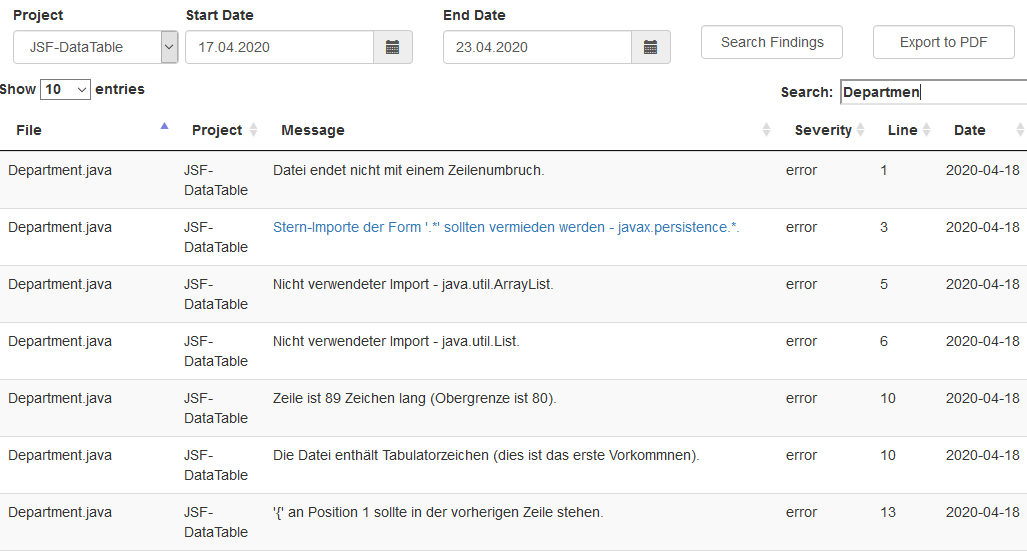
\includegraphics[height=8cm]{images/tableRec.PNG}
  % The short caption should be capitalised
  % The full caption should hold a full sentence. 
 \caption[Am häufigsten vorkommende Fehler in den ausgewählten Projekten.]{Am meisten vorkommende Fehler in den ausgewählten Projekten. (vgl. Fehler in den den Abbildungen \ref{fig:findingsInIDE} und \ref{fig:checkstyleHTMLReport})}
  \label{fig:tableRec}
\end{figure}

\item Durch das Plugin können eine Vielzahl an Tools unterstützt und eingebunden werden. Die einzige Voraussetzung hierbei ist das Angeben der XML-Results. Dadurch können die Benutzer die Applikation individuell gestalten, da nur die von ihnen gewünschten Fehler und Bugs analysiert werden können. Ein Einsatz beliebiger Tools für spezifische Probleme kann so unterstützt werden (siehe Punkt 2.3). Herkömmliche Lösungen wie Veracode oder SonarQube verwenden eine eingebaute und vorgegebene Code Analyse.
\item Aufgrund der Verwendung einer Web-Applikation ist das Springen, automatische Ausbessern und Navigieren zu den Fehlern, im Unterschied zu Entwicklungsumgebungen, nicht möglich. Die Fehler werden daher auch nicht direkt in der Entwicklungsumgebung markiert.
\item Im Frontend können Meldungen gezielt ignoriert werden (siehe Punkt 4.6.2.5). Dazu muss die bestimmte Meldung angegeben werden. In anderen Lösungen gibt es verschiedene Konzepte für diese Funktion, zum Beispiel das Hinzufügen von bestimmten Modulen mit denen man im Code Fehler ignorieren kann, mit Annotations oder mit Kommentaren. In anderen Lösungen können auch Code-Blöcke für die Analyse ausgenommen werden.
\item Mit dem Hinzufügen von Recommendations können Fehler vermieden werden (siehe Recommendation-Link in Abbildung \ref{fig:tableRec}). Das Ziel hierbei ist es auch, einen Lernprozess bei den Benutzerinnen und Benutzern zu ermöglichen. Herkömmliche Lösungen ermöglichen das automatische Ausbessern der Fehler oder geben zusätzliche  Informationen bei den Meldungen an.



\item Im Frontend können verschiedene Charts zur Unterstützung angezeigt werden. Auch andere Web-Lösungen wie SonarQube und Veracode ermöglichen das Anzeigen von Charts mit Informationen wie Anzahl der Fehlertypen oder Charts zur Komplexität der Fehler. In Entwicklungsumgebungen werden hingegen keine Charts angezeigt.
\end{itemize}
\section{Evaluierungen der Webapplikation mit Testpersonen} 
Die einzelnen Kriterien in den Beschreibungen der Evaluierung der Testpersonen werden im Punkt 1.2.2 genauer beschrieben. 

Die Testpersonen bewerten die einzelnen Punkte mit den Noten 1-5. Anmerkungen der Testpersonen werden zur Bewertung angegeben. Beim Kriterium \textit{Unterstützung} suchen die Testpersonen bestimmte Fehler  mithilfe der Applikation und bewerten die Fehlersuche im Vergleich zu herkömmlichen Lösungen bzw. zu einer freien Fehlersuche.
\subsubsection{Testpersonen}
\textbf{Testperson 1} \\
Erfahrung in der Softwareentwicklung: 5 Jahre Berufserfahrung; Erfahrung mit der Statischen Code Analyse: Bereits eingesetzt und verwendet \\
Bewertung der Kriterien:

Einfachheit: 2, Sub-Pages (Projekt, Charts, Suche, Übersicht) für eine bessere Unterteilung der Informationen \newline Übersicht: 2, Es sollte die Möglichkeit bestehen, einzelne Fehler genauer zu folgen, zum Beispiel wann genau der Fehler erstellt wurde. \newline  Unterstützung: 1, Fehler konnte in unter fünfzehn Sekunden gefunden werden, Besonders in Teams ist eine Git-Unterstützung notwendig um genauere Analysen und Informationen über die Entwickler zu bekommen.  \newline  Individualität: 1 \newline  Performance: 1 \newline  Verständnis: 2 \newline 

\textbf{Testperson 2} \\
Erfahrung in der Softwareentwicklung: 2 Jahre Berufserfahrung; Erfahrung mit der Statischen Code Analyse: Keine Erfahrungen\\
Bewertung der Kriterien:

Einfachheit: 3, Erstellung einer Dokumentation und Beispielen um die Verwendung des Programms (Plugins) genauer verstehen zu können. \newline  Übersicht: 1 \newline  Unterstützung: 2, Fehler konnte in unter zwanzig Sekunden gefunden werden; Hinzufügen einer Fehler-Historie, um Fehler genau verfolgen zu können und um Fragen beantworten zu können wie: Wann ist der Fehler das erste Mal aufgetreten? Wie lange war der Fehler im Projekt? \newline  Individualität: 1 \newline  Performance: 1 \newline  Verständnis: 1 \newline 

\textbf{Testperson 3} \\
Erfahrung in der Softwareentwicklung: 4 Jahre Berufserfahrung; Erfahrung mit der Statischen Code Analyse: Bereits eingesetzt und wird aktuell verwendet\\
Bewertung der Kriterien:

Einfachheit: 2, Mit einer Desktop-Applikation kann eine bessere Interaktion mit der Entwicklungsumgebung erfolgen \newline Übersicht: 1 \newline  Unterstützung: 1, Fehler konnte in unter fünfzehn Sekunden gefunden werden \newline Individualität: 2, Möglichkeit zur eigenen weiteren Einteilung der Fehler in Kategorien würde die Übersicht und die Individualität in der Webapplikation steigern.  \newline Performance: 1 \newline  Verständnis: 2, Angabe des eingesetzten Tools bei der Meldung\newline 

\textbf{Testperson 4} \\
Erfahrung in der Softwareentwicklung: 1 Jahr Berufserfahrung; Erfahrung mit der Statischen Code Analyse: Keine Erfahrungen\\
Bewertung der Kriterien:

Einfachheit: 3, Hinzufügen einer Dokumentation für das Einfügen der Plugins.  \newline Übersicht: 1 \newline  Unterstützung: 1, Fehler konnte in unter zwanzig Sekunden gefunden werden \newline Individualität: 2, Severity (Fehlerlevel) soll vom Benutzer auch selbst bestimmt werden können\newline Performance: 1 \newline  Verständnis: 2\newline 

\textbf{Testperson 5} \\
Erfahrung in der Softwareentwicklung: 2 Jahre Berufserfahrung; Erfahrung mit der Statischen Code Analyse: Bereits eingesetzt\\
Bewertung der Kriterien:

Einfachheit: 2, Hinzufügen einer Dokumentation für das Einfügen der Plugins.  \newline Übersicht: 2, Charts sollen in Pop-Ups angezeigt werden. Tabelle soll nach Packages gefiltert werden können \newline  Unterstützung: 1, Fehler konnte in unter fünfzehn Sekunden gefunden werden \newline Individualität: 1 \newline Performance: 1 \newline  Verständnis: 2, Bessere Erklärungen zu den Charts und zu den Feldern in der Tabelle (Schwere des Fehlers)\newline 

\textbf{Testperson 6} \\
Erfahrung in der Softwareentwicklung: 7 Jahre Berufserfahrung; Erfahrung mit der Statischen Code Analyse: Bereits eingesetzt und wird aktuell verwendet\\
Bewertung der Kriterien:

Einfachheit: 3, Hinzufügen einer Dokumentation für das Einfügen der Plugins; Erstellen von Container für die Docker-Unterstützung um die Applikation und die Datenbank schnell und einfach verwenden zu können; Erstellen einer Git-Integration und Möglichkeit zur Öffnung der Files in Github um die Fehler und Bugs direkt einsehen zu können \newline Übersicht: 2, Navigation zu den einzelnen Sections, Pfade der Klassen anzeigen, Zusätzlich zur Datum-Filterung auch Möglichkeit der Filterung nach Commit \newline  Unterstützung: 1, Fehler konnte in unter fünfzehn Sekunden gefunden werden \newline Individualität: 1, Erstellen eines Security-Tokens für die Sicherheit in der Applikation \newline Performance: 1 \newline  Verständnis: 1\newline 

\subsubsection{Interpretation der Evaluierungen}
\textbf{Einfachheit}
Durchschnittlicher Wert: 2,5\\
Die meisten Testpersonen, besonders Entwicklerinnen und Entwickler mit wenig Berufserfahrung, wiesen auf eine fehlende Dokumentation hin, insbesondere beim Einfügen und bei der Verwendung des Plugins. Eine Dokumentation und Beschreibung kann bei Tools wie Github hinzugefügt werden. Auch in der Webapplikation können Tooltips und Hilfe-Seiten für die Benutzung des Plugins hinzugefügt werden.

\textbf{Übersicht}
Durchschnittlicher Wert: 1,5\\
Bei diesem Kriterium erwähnten mehrere Testpersonen die Aufteilung der Applikation in mehrere Unter-Seiten. Ebenso eine genauere Betrachtung und Anzeige der Fehler und Charts(Historie und Pop-ups), könnte die Bewertung der Übersicht weiter steigern.

\textbf{Unterstützung}
Durchschnittlicher Wert: 1,2\\
Die hohe Bewertung bei der Unterstützung bestätigt die Möglichkeit zur Verbesserung des Codes der Entwicklerinnen und Entwickler. Einige Testpersonen erwähnten die Integration mit Tools für die Versionsverwaltung, um auch Team-Unterstützung integrieren zu können.

\textbf{Individualität}
Durchschnittlicher Wert: 1,4\\
Die Möglichkeit, verschiedene Tools für die Statische Code Analyse integrieren zu können, war ausschlaggebend für die Bewertung beim Kriterium der Individualität. Weitere Funktionalitäten wie die eigene Einteilung der Fehler in Kategorien und die Möglichkeit zur Erstellen eines Passworts für die Sicherung der Webapplikation würde die Individualität weiter steigern.

\textbf{Performance}
Durchschnittlicher Wert: 1,2\\
Der Wert der Performance zeigt, dass bei der Evaluierung keine größeren Performance-Probleme aufgetreten sind. Hierbei muss aber auch die Infrastruktur und die Menge der Daten bemerkt werden, die in der Praxis auch abweichen und so die Performance beeinflussen können.

\textbf{Verständnis}
Durchschnittlicher Wert: 1,7\\
Weitere Erklärungen zu den einzelnen Feldern in der Tabelle und zu den Charts könnten das Verständnis der Präsentationen der Daten verbessern.     % evaluation of prototype
%%%%%%%%%%%%%%%%%%%%%%%%%%%%%%%%%%%%%%%%%%%%%%%%%%%%%%%%%%%%%%%%%%%%%%%%%%%%%
\chapter{Conclusion and Outlook}
\label{chap:conclusion}
%%%%%%%%%%%%%%%%%%%%%%%%%%%%%%%%%%%%%%%%%%%%%%%%%%%%%%%%%%%%%%%%%%%%%%%%%%%%%
\chapterstart

Your text here\ldots
Sum up the results achieved. State current limitations of your solution. Suggest further research by explaining how others could built on your results.

\chapterend



%%
% Hints by Daniela Holzer 2017
% "instructions for composing degree papers.pdf"
%
% Formal Guidelines
%   Diploma thesis: 17 000 words ± 10% (excluding appendix)
%   Each of the two Bachelor papers: 10 000 words ± 10% (excluding appendix)
%%      % summary, your conclusions/outlook

%\appendix
%%%%%%%%%%%%%%%%%%%%%%%%%%%%%%%%%%%%%%%%%%%%%%%%%%%%%%%%%%%%%%%%%%%%%%%%%%%%%%
\chapter*{Acronyms} % Note the * with \chapter*, which hides it from TOC
\label{chap:acronyms}
%%%%%%%%%%%%%%%%%%%%%%%%%%%%%%%%%%%%%%%%%%%%%%%%%%%%%%%%%%%%%%%%%%%%%%%%%%%%%
% Which one will be the longest ...?
% ABCDE --> \begin{acronym}[ABCDE]
\footnotesize
\begin{acronym}[ABCDE]
  \acro{SQL} {Structured Query Language}
\end{acronym}
\normalsize
       % optional

%\TODO{Finally, check the bibliography. Are you sure, that everyone can find the given resources with the information you supplied? Besides author and  year, for books you need the publisher information and the ISBN, for IEEE/ACM research papers add the conference title, location and the DOI.}
\printbibliography

% Adding entry "References" to TOC
% LaTeX-Note: this entry must be added after \printbibliography
%             to get a working link in the TOC!
\addcontentsline{toc}{chapter}{References}

\end{document}


%**********************************************************************
%**********************************************************************
